We proceed to establish consistency for the estimators introduced in the previous
section. For the brevity of the presentation, we only focus on the MWM method;
consistency for MWMS can be obtained in a similar fashion. 
Fix $m$, and assume that $P^{j}$ is the 
true distribution of data $X_{j,i}$ for $j = 1,\ldots,m$. Write
$\vec{G}=(G_{1},\ldots,G_{m})$ and $\vec{n}=(n_{1},\ldots,n_{m})$. We say 
$\vec{n} \to \infty$ if $n_{j} \to \infty$ for $j=1,\ldots, m$. Define the following 
functions
\vspace{-6pt}
\begin{eqnarray}
f_{\vec{n}}(\vec{G},\Hcal)=\mathop {\sum }\limits_{j=1}^{m}{W_{2}^{2}(G_{j},P_{n_{j}}^{j})}+W_{2}^{2}(\Hcal,\dfrac{1}{m}\mathop {\sum }\limits_{j=1}^{m}{\delta_{G_{j}}}), \nonumber \\
f(\vec{G},\Hcal)=\mathop {\sum }\limits_{j=1}^{m}{W_{2}^{2}(G_{j},P^{j})}+W_{2}^{2}(\Hcal,\dfrac{1}{m}\mathop {\sum }\limits_{j=1}^{m}{\delta_{G_{j}}}), \nonumber
\end{eqnarray}
where $G_{j} \in \mathcal{O}_{k_{j}}(\Theta)$, $\Hcal \in \mathcal{E}_{M}(\mathcal{P}(\Theta))$ as $1 \leq j \leq m$. 
The first consistency property of the WMW formulation:
\begin{theorem} \label{theorem:objective_consistency_multilevel_Wasserstein_means} 
Given that $P^{j} \in \mathcal{P}_{2}(\Theta)$ for $1 \leq j \leq m$. Then,
there holds almost surely, as $\vec{n} \to \infty$
\vspace{-6pt}
\begin{eqnarray}
\mathop {\inf }\limits_{\substack {G_{j} \in \mathcal{O}_{k_{j}}(\Theta), \\ \Hcal \in \mathcal{E}_{M}(\mathcal{P}_{2}(\Theta))}}f_{\vec{n}}(\vec{G},\Hcal) - \mathop {\inf }\limits_{\substack {G_{j} \in \mathcal{O}_{k_{j}}(\Theta), \\ \Hcal \in \mathcal{E}_{M}(\mathcal{P}_{2}(\Theta))}}f(\vec{G},\Hcal) \rightarrow 0. \nonumber
\end{eqnarray}

\end{theorem}
The next theorem establishes that the ``true'' global and local clusters can be
recovered. To this end, assume that for each $\vec{n}$ there is an optimal solution $
(\widehat{G}_{1}^{n_{1}},\ldots,\widehat{G}_{m}^{n_{m}},\widehat{\Hcal}^{\vec{n}})$ or in 
short $(\vec{\widehat{G}}^{\vec{n}},\Hcal^{\vec{n}})$ of the objective function 
\eqref{eqn:multilevel_Kmeans_typeone}. Moreover, there exist a (not necessarily unique)
optimal solution minimizing $f(\vec{G},\Hcal)$ over $G_{j} \in \mathcal{O}_{k_{j}}(\Theta)$ and $\Hcal \in 
\mathcal{E}_{M}(\mathcal{P}_{2}(\Theta))$. Let $\mathcal{F}$ be the collection 
of such optimal solutions. For any $G_{j} \in \mathcal{O}_{k_{j}}(\Theta)$ and $\Hcal \in 
\mathcal{E}_{M}(\mathcal{P}_{2}(\Theta))$, define
\vspace{-6pt}
\begin{eqnarray}
d(\vec{G},\Hcal,\mathcal{F})=\inf \limits_{(\vec{G}^{0}, \Hcal^{0}) \in \mathcal{F}}\sum \limits_{j=1}^{m}{W_{2}^{2}(G_{j},G_{j}^{0})} \nonumber
+W_{2}^{2}(\Hcal,\Hcal^{0}). \nonumber
\end{eqnarray}
Given the above assumptions, we have the following result regarding the convergence of $(\widehat{\vec{G}}^{\vec{n}},\Hcal^{\vec{n}})$:
\begin{theorem} \label{theorem:convergence_measures_multilevel_Wasserstein_means}
Assume that $\Theta$ is bounded and $P^{j} \in \mathcal{P}_{2}(\Theta)$ for all $1 \leq j 
\leq m$. Then, we have $d(\vec{\widehat{G}}^{\vec{n}},\widehat{\Hcal}
^{\vec{n}},\mathcal{F}) \to 0$ as $\vec{n} \to \infty$ almost surely.
\end{theorem}
\paragraph{Remark:}(i) The assumption $\Theta$ is bounded is just for the convenience of 
proof argument. We believe that the conclusion of this theorem may still hold when $\Theta 
= \mathbb{R}^{d}$. (ii) If $|\mathcal{F}|=1$, i.e., there exists an unique optimal solution $
\vec{G}^{0},\Hcal^{0}$ minimizing $f(\vec{G},\Hcal)$ over $G_{j} \in \mathcal{O}_{k_{j}}(\Theta)
$ and $\Hcal \in \mathcal{E}_{M}(\mathcal{P}_{2}(\Theta))$, the result of Theorem 
\ref{theorem:convergence_measures_multilevel_Wasserstein_means} implies that $W_{2}
(\widehat{G}_{j}^{n_{j}},G_{j}^{0}) \to 0$ for $1 \leq j \leq m$ and $W_{2}(\widehat{\Hcal}
^{\vec{n}},\Hcal^{0}) \to 0$ as $\vec{n} \to \infty$.

\begin{figure*}[ht]
%\vskip 0.2in
\centerline{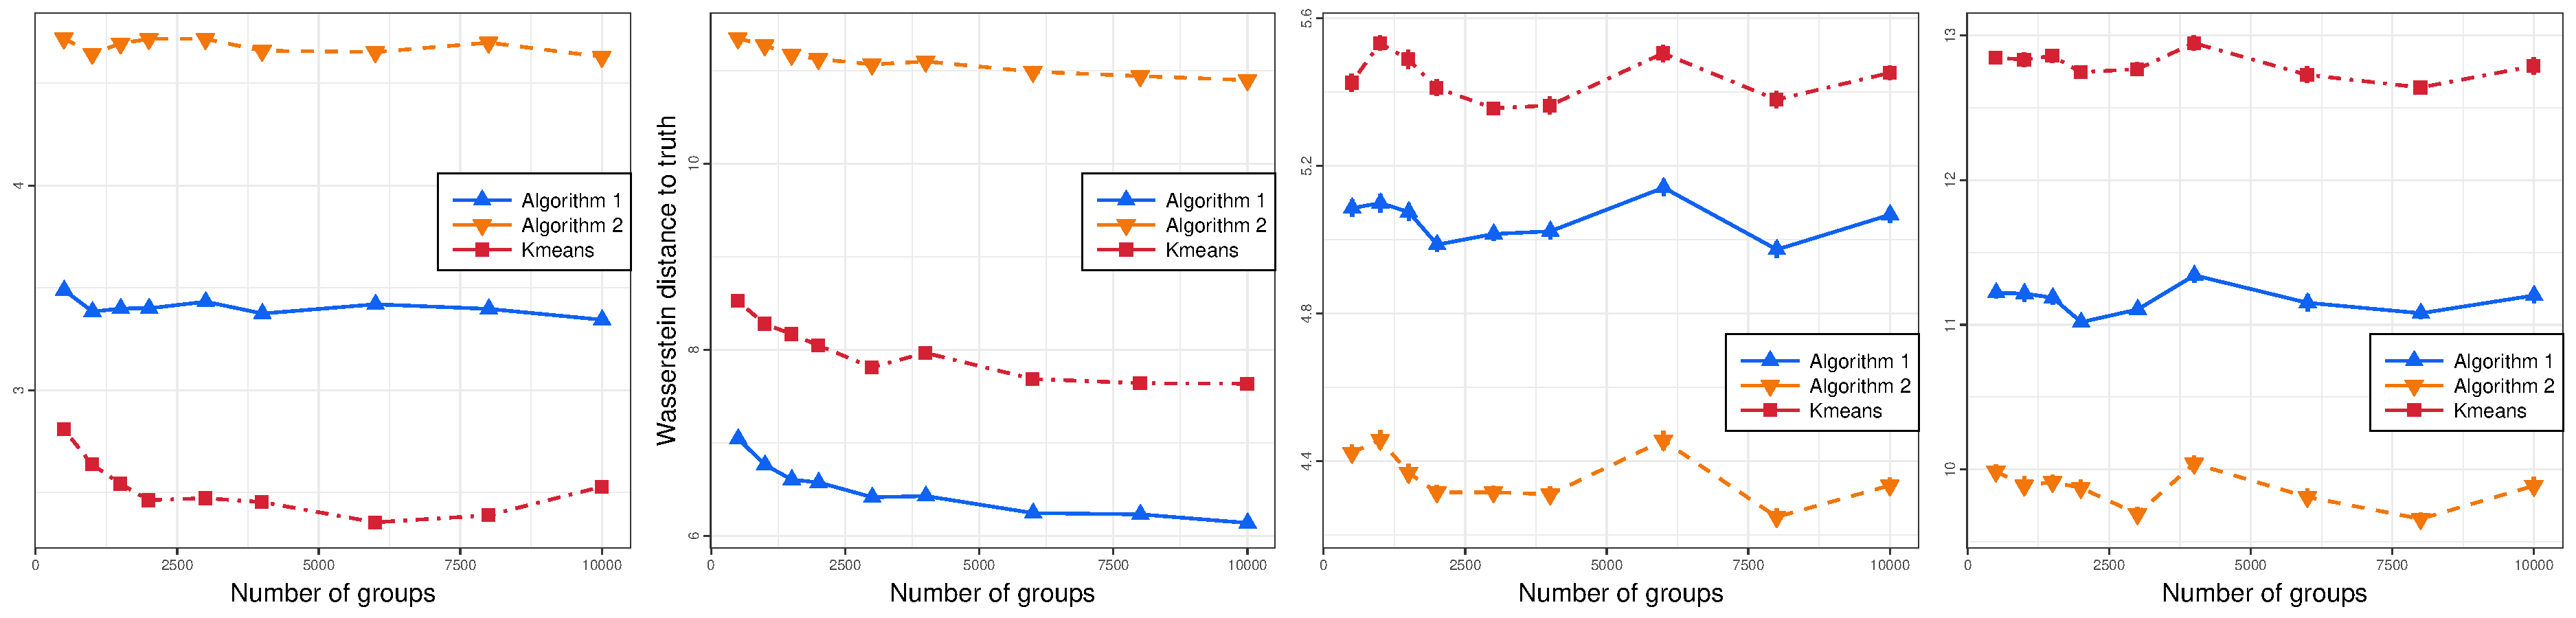
\includegraphics[width=0.9\textwidth]{M_compare.pdf}}
\caption{Data with a lot of small groups: (a) NC data with constant variance; (b) NC data with non-constant variance; (c)
LC data with constant variance; (d) LC data with non-constant variance}
%\caption{No constraint experiment (left); Local constraint experiment (right)}
\label{fig:simul_M}
\end{figure*}

\begin{figure*}[ht]
\centerline{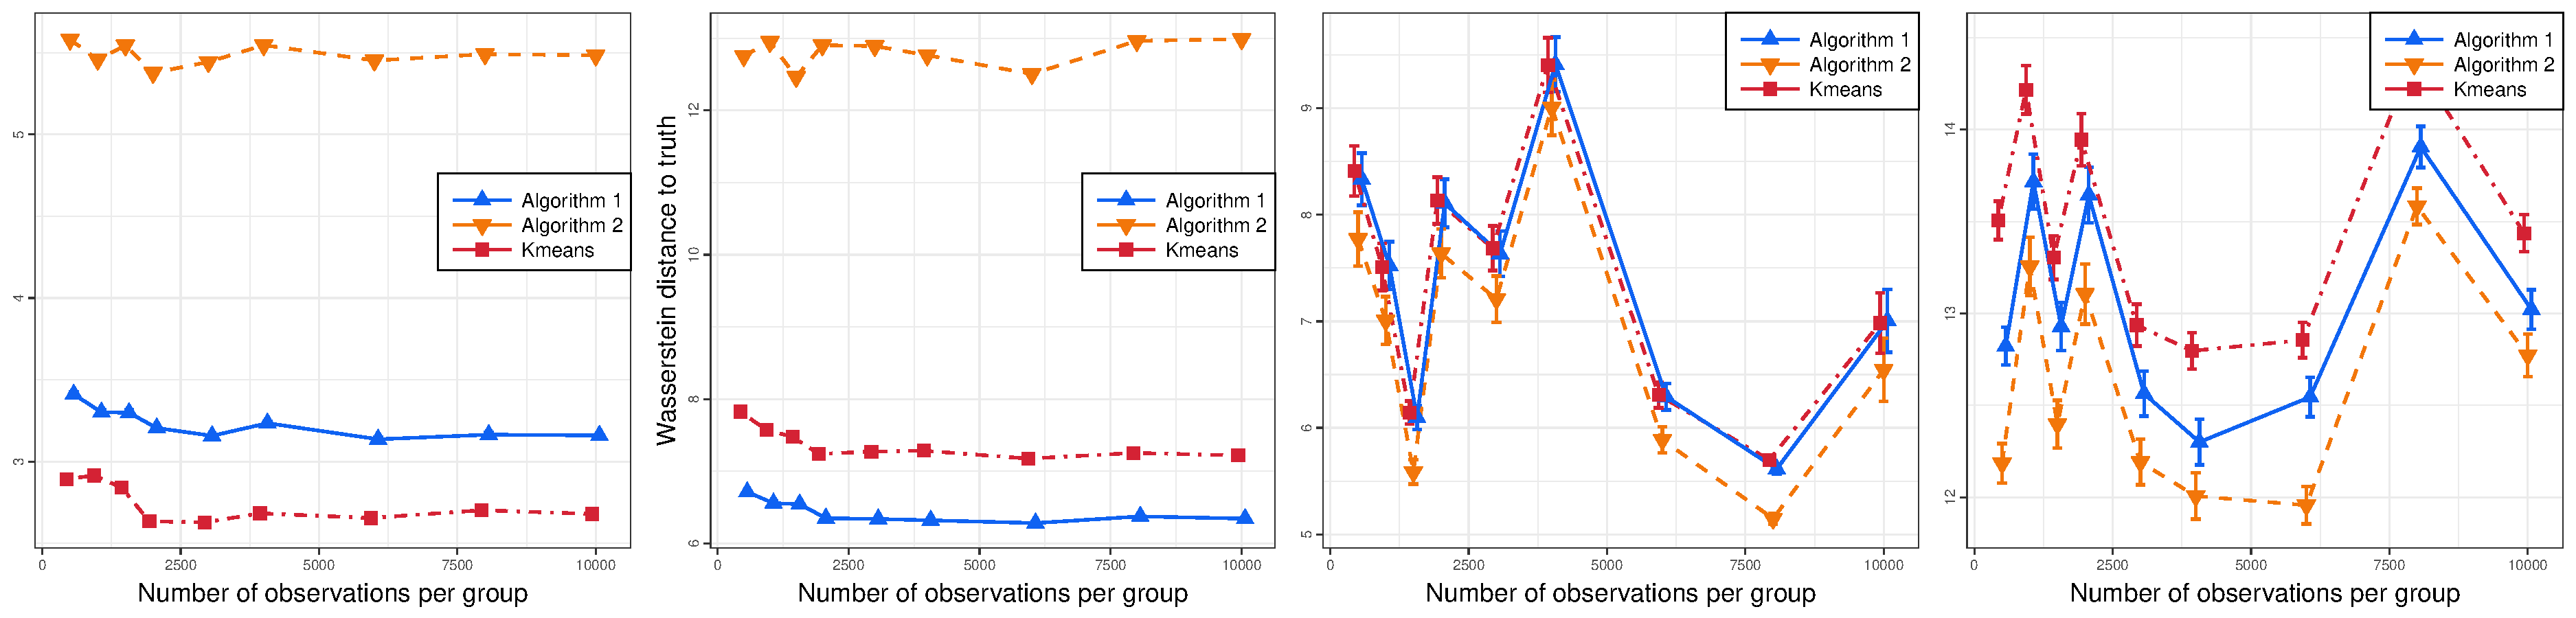
\includegraphics[width=0.9 \textwidth]{N_compare.pdf}}
\caption{Data with few big groups: (a) NC data with constant variance; (b) NC data with non-constant variance; (c) LC
data with constant variance; (d) LC data with non-constant variance}
\label{fig:simul_N}
\end{figure*}
